%% ════════════════════════════════════════════════════════════════════════════
\section{Results}
\label{sec:results}

\subsection{Empirical Audit of Leakage Inflation}
\label{sec:leakage_results}
Table~\ref{tab:leakage_inflation} presents model performance in Ahmedabad across Setups~A, B, and C, examining performance differences across evaluation setups and visualising the primary full-window trajectories (Figure~\ref{fig:leakage_inflation}).

\begin{table}[htbp]
\centering
\resizebox{\linewidth}{!}{
\begin{tabular}{l cccccc c}
\toprule
 & \multicolumn{2}{c}{\textbf{Setup A (Random)}} & \multicolumn{2}{c}{\textbf{Setup B (Chrono)}} & \multicolumn{2}{c}{\textbf{Setup C (Rolling)}} & \\
\cmidrule(lr){2-3} \cmidrule(lr){4-5} \cmidrule(lr){6-7}
\textbf{Model} & \textbf{MAE} & $\mathbf{R^2}$ & \textbf{MAE} & $\mathbf{R^2}$ & \textbf{MAE} & $\mathbf{R^2}$ & $\Delta R^2 \text{ (A$-$B)}$ \\
\midrule
\multicolumn{8}{l}{\textit{Panel A: Primary full-window runs (Setup A/B $n_{\text{test}}=230$, Setup C $n_{\text{test}}=507$):}} \\
Ridge & 24.99 & 0.715 & 30.07 & 0.166 & 20.83 & 0.520 & +0.548 \\
Random Forest & 18.50 & 0.815 & 30.49 & 0.015 & 20.73 & 0.505 & +0.800 \\
XGBoost & 19.12 & 0.814 & 26.34 & 0.386 & 20.91 & 0.493 & +0.428 \\
\midrule
\multicolumn{8}{l}{\textit{Panel B: Excluding 89 March--May 2020 days (Setup A $n_{\text{test}}=212$, Setup B $n_{\text{test}}=141$, Setup C $n_{\text{test}}=141$):}} \\
Ridge (excl.\ Mar--May 2020) & 22.09 & 0.776 & 22.01 & 0.665 & 47.32 & -0.299 & +0.111 \\
Random Forest (excl.\ Mar--May 2020) & 17.61 & 0.829 & 18.01 & 0.747 & 39.33 & 0.145 & +0.082 \\
XGBoost (excl.\ Mar--May 2020) & 17.99 & 0.833 & 19.74 & 0.731 & 39.78 & 0.142 & +0.102 \\
\midrule
\multicolumn{8}{l}{\textit{Panel C: Like-for-like Setup C on Setup B's full 230-day window (2019-10-24 to 2020-07-01):}} \\
Ridge (230d Setup B window) & -- & -- & 30.07 & 0.166 & 41.77 & -0.111 & -- \\
Random Forest (230d Setup B window) & -- & -- & 30.49 & 0.015 & 37.78 & 0.120 & -- \\
XGBoost (230d Setup B window) & -- & -- & 26.34 & 0.386 & 38.65 & 0.111 & -- \\
\bottomrule
\end{tabular}
}
\caption{Empirical Leakage Inflation in Ahmedabad: Setup A (Random) vs Setup B (Chrono) vs Setup C (Rolling-Origin). Panel~A shows primary full-window runs. Panel~B excludes the 89 valid March--May 2020 days across all three setups (141-day Persistence MAE $= 42.04$). Panel~C evaluates Setup~C on Setup~B's exact 230-day window (230-day Persistence MAE $= 33.31$).}
\label{tab:leakage_inflation}
\end{table}


\begin{figure}[htbp]
  \centering
  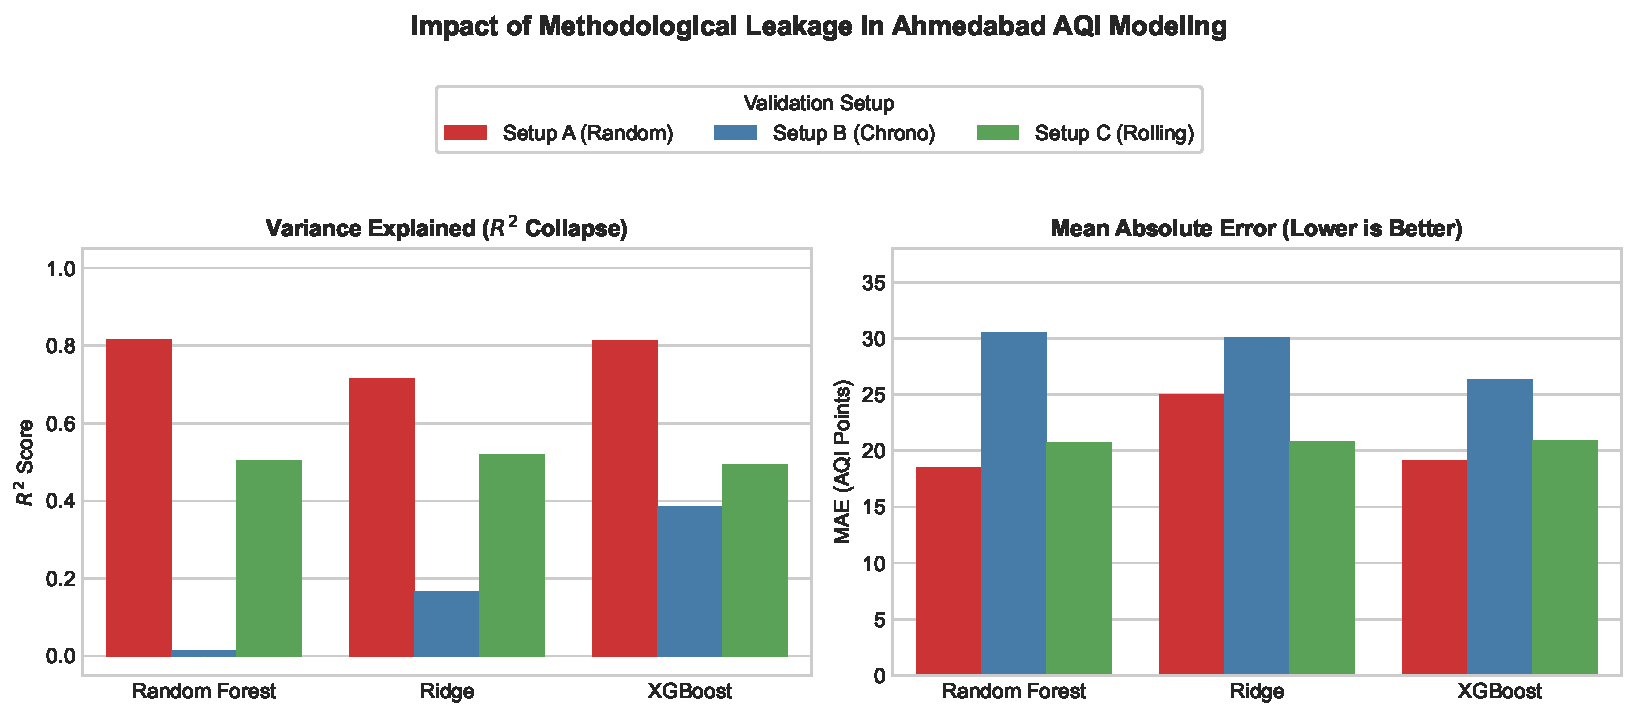
\includegraphics[width=0.88\textwidth]{../results/figures/fig1_leakage_inflation.pdf}
  \caption{Primary full-window leakage audit in Ahmedabad across Setups~A, B, and C for $R^2$ (left) and MAE (right). Lockdown-excluded Setup~A/B and like-for-like 230-day Setup~C sensitivity rows are reported in Table~\ref{tab:leakage_inflation}.}
  \label{fig:leakage_inflation}
\end{figure}

The comparison between Setup~A and Setup~B shows how strongly temporal regime shifts affect concurrent-input models. In Setup~A (random splitting with concurrent inputs, 10 seeds, $n_{\text{train}} = 919$, $n_{\text{test}} = 230$, covering only days with valid PM$_{2.5}$ observations), Random Forest achieved a mean $R^2$ of $\mathbf{0.815 \pm 0.047}$ (mean MAE $= 18.50 \pm 1.64$ across seeds). Because Setups A and B are both restricted to the 1,149 Ahmedabad days with valid PM$_{2.5}$ measurements, the Setup~B test observations have \emph{observed} (not imputed) pollutant inputs. When arranged chronologically (Setup~B, $n_{\text{train}} = 919$, $n_{\text{test}} = 230$), Random Forest dropped to $R^2 = \mathbf{0.015}$ ($\text{MAE} = 30.49$) and Ridge to $R^2 = 0.166$ ($\text{MAE} = 30.07$). Crucially, Setup~B's test window (2019-10-24 to 2020-07-01) spans India's COVID-19 lockdown (which began 25 March 2020, sharply reducing ambient AQI \cite{mahato2020}). Of the 92 calendar days in March--May 2020, 89 have valid PM$_{2.5}$ and AQI records. Excluding those 89 lockdown days restores Setup~B ($n_{\text{test}} = 141$) to $R^2 = 0.747$ ($\text{MAE} = 18.01$) for Random Forest, $R^2 = 0.665$ ($\text{MAE} = 22.01$) for Ridge, and $R^2 = 0.731$ ($\text{MAE} = 19.74$) for XGBoost. Running Setup~A on the same 1,060 non-lockdown days ($n_{\text{test}} = 212$, 10 seeds) gives $\text{MAE} = 17.61 \pm 1.15$ ($R^2 = 0.829 \pm 0.041$) for Random Forest, $22.09 \pm 0.99$ ($R^2 = 0.776 \pm 0.043$) for Ridge, and $17.99 \pm 1.11$ ($R^2 = 0.833 \pm 0.037$) for XGBoost. Thus, on non-lockdown days random-split MAE inflation is small, and the remaining $\Delta R^2$ gap is at most an upper bound because $R^2$ depends on test-set variance; the primary `0.815 -> 0.015` collapse was driven mainly by the COVID-19 lockdown regime shift.

\textbf{Like-for-like Setup B vs. C comparison:} Primary Setup~B uses $n_{\text{test}} = 230$ days (2019-10-24 to 2020-07-01), whereas primary Setup~C uses $n_{\text{test}} = 507$ days (2022-08-09 to 2023-12-30; zero overlapping dates). To provide a like-for-like concurrent-vs-lagged comparison, we also evaluated Setup~C on Setup~B's exact 230-day window (Table~\ref{tab:leakage_inflation}): Persistence achieved $\text{MAE} = 33.31$ ($R^2 = 0.131$), whereas strictly lagged Random Forest ($\text{MAE} = 37.78$), XGBoost ($38.65$), and Ridge ($41.77$) all trailed Persistence. On the 141 non-lockdown subset, concurrent-input Setup~B Random Forest ($\text{MAE} = 18.01$) strongly outperformed lagged Setup~C Random Forest ($\text{MAE} = 39.33$; Persistence $42.04$), isolating the large inflation caused by concurrent same-day pollutant inputs.

\subsection{Leak-Free Next-Day Benchmark (\texorpdfstring{$h=1$}{h=1})}
\label{sec:h1_results}
Table~\ref{tab:main_benchmark_h1} documents next-day forecasting performance under leak-free Setup~C for the two anchor cities (Ahmedabad and Chennai), including 95\% moving block-bootstrap confidence intervals, alongside model MAE distributions across all six cities (Figure~\ref{fig:model_comparison}).

\begin{table}[htbp]
\centering
\caption{Setup C Next-Day ($t+1$) Forecasting Benchmark vs Persistence Baseline. \textit{Note:} Skill score denotes normalized MAE improvement over Persistence ($1 - \text{MAE}_{\text{model}}/\text{MAE}_{\text{persistence}}$); DM $p$-value evaluates two-tailed significance vs Persistence, with asterisks ($^*$) marking $p < 0.05$ in either direction (both candidate model wins and Persistence wins).}
\label{tab:main_benchmark_h1}
\resizebox{\linewidth}{!}{\begin{tabular}{llcccccc}
\toprule
City & Model & MAE & RMSE & R2 & Skill & Band Acc (\%) & DM p-value \\
\midrule
Ahmedabad & Persistence & 20.21 & 28.83 & 0.462 & 0.000 & 75.8 & -- \\
Ahmedabad & Seasonal Naive & 26.85 & 35.95 & 0.162 & -0.328 & 70.0 & 0.000$^*$ \\
Ahmedabad & Moving Average & 20.01 & 27.10 & 0.525 & 0.010 & 76.7 & 0.766 \\
Ahmedabad & Ridge & 20.83 & 27.24 & 0.520 & -0.031 & 77.5 & 0.402 \\
Ahmedabad & Random Forest & 20.73 & 27.67 & 0.505 & -0.026 & 79.5 & 0.510 \\
Ahmedabad & XGBoost & 20.91 & 28.01 & 0.493 & -0.034 & 78.7 & 0.419 \\
Chennai & Persistence & 17.90 & 28.58 & -0.034 & 0.000 & 74.4 & -- \\
Chennai & Seasonal Naive & 23.02 & 35.78 & -0.620 & -0.286 & 67.9 & 0.000$^*$ \\
Chennai & Moving Average & 18.37 & 28.48 & -0.026 & -0.026 & 72.4 & 0.494 \\
Chennai & Ridge & 16.18 & 25.05 & 0.206 & 0.096 & 78.0 & 0.010$^*$ \\
Chennai & Random Forest & 15.84 & 24.87 & 0.218 & 0.115 & 78.0 & 0.002$^*$ \\
Chennai & XGBoost & 16.11 & 25.34 & 0.188 & 0.100 & 76.9 & 0.001$^*$ \\
\bottomrule
\end{tabular}}
\end{table}


\begin{figure}[htbp]
  \centering
  \includegraphics[width=0.88\textwidth]{../results/figures/fig2_model_comparison_h1.pdf}
  \caption{Next-day ($h=1$) MAE across models and cities under Setup~C. All machine learning models fail to significantly surpass Persistence except in coastal Chennai.}
  \label{fig:model_comparison}
\end{figure}

\paragraph{Ahmedabad.}
The naive Persistence baseline achieved an MAE of \textbf{20.21} ($R^2 = 0.462$). While the 7-day Moving Average achieved an MAE of \textbf{20.01} ($+1.0\%$ skill), this difference was statistically indistinguishable from zero ($p = 0.766$ via Diebold-Mariano). Crucially, every evaluated machine learning model (Random Forest, XGBoost, and Ridge Regression) yielded negative skill scores relative to Persistence: Random Forest attained $\text{MAE} = 20.73$ ($\text{Skill} = -0.026, p = 0.510$), Ridge attained $\text{MAE} = 20.83$ ($\text{Skill} = -0.031, p = 0.402$), and XGBoost attained $\text{MAE} = 20.91$ ($\text{Skill} = -0.034, p = 0.419$). Under the Diebold-Mariano test (no HAC correction at $h=1$, $k=0$; $p > 0.40$), none of the machine learning forecasters statistically significantly outperformed the naive Persistence baseline.

\paragraph{Chennai.}
Chennai exhibited a fundamentally different atmospheric regime. In this coastal metropolis, Persistence performed poorly ($\text{Persistence } R^2 = -0.034, \text{MAE} = 17.90$), consistent with the hypothesis that maritime circulation weakens day-to-day AQI inertia. Machine learning models established statistically significant predictive skill: Random Forest reduced MAE to \textbf{15.84} ($+11.5\%$ skill, $p = 0.002$), XGBoost achieved $\text{MAE} = 16.11$ ($+10.0\%$ skill, $p = 0.001$), and Ridge attained $\text{MAE} = 16.18$ ($+9.6\%$ skill, $p = 0.010$). Note that although the marginal 95\% block-bootstrap CIs overlap (e.g., Persistence $[15.14, 21.11]$ vs.\ Random Forest $[13.39, 18.71]$), the paired Diebold-Mariano test evaluates day-by-day loss differentials and is therefore more powerful than comparing marginal confidence intervals. Because Kaggle pollutant records end in 2020, all 28 pollutant-lag columns are imputed during Chennai's 2022--2023 test window, meaning this skill derives from AQI lags, rolling AQI statistics, and calendar harmonics alone. None of these $h=1$ Chennai results survive Bonferroni correction ($\alpha = 0.05/60 = 0.00083$) under $k=0$ (though XGBoost would survive under the $k=3$ sensitivity check at $p = 0.00075$). In a 21-column AQI-only ablation dropping the 28 pollutant-lag columns, Ahmedabad ML still failed to beat Persistence (Ridge $21.17$, RF $21.33$, XGBoost $21.24$; all $p \ge 0.168$), while Chennai retained positive skill for Ridge ($16.41, p = 0.016$) and XGBoost ($16.62, p = 0.019$), with Random Forest dropping to $16.84$ ($p = 0.087$).

\subsection{Cross-City Evaluation Across Gujarat}
\label{sec:multicity_results}
Table~\ref{tab:cross_city_mae} expands the leak-free Setup~C next-day benchmark across all six evaluated cities.

\input{../results/tables/table4_multicity.tex}

Cross-city analysis reveals three distinct operational regimes:
\begin{enumerate}
  \item \textbf{Simple-Baseline Dominance (Ahmedabad, Gandhinagar):} In urban continental Gujarat, strong day-to-day autocorrelation ($\rho_1 > 0.75$; Ahmedabad 0.75, Gandhinagar 0.83) renders simple classical baselines highly competitive, and ML models fail to outperform them. In Gandhinagar, Ridge Regression achieved $\text{MAE} = 23.43$ versus Persistence $\text{MAE} = 23.88$ ($p = 0.590$); Random Forest and XGBoost performed worse than Persistence ($p = 0.143$ and $p = 0.539$), whereas simple ARIMA(1,0,0) achieved $\text{MAE} = 22.64$ ($p = 0.0005$; Table~\ref{tab:extra_baselines}).
  \item \textbf{Persistence Superiority (Vapi):} In the chemical industrial corridor of Vapi, Persistence ($\text{MAE} = \mathbf{18.98}, R^2 = 0.813$) was \emph{statistically significantly superior} to all five candidate models at $h=1$: Seasonal Naive ($p = 7.3 \times 10^{-7}$), Moving Average ($p = 0.012$), Random Forest ($p = 7.9 \times 10^{-5}$), XGBoost ($p = 0.0009$), and Ridge ($p = 0.003$). We hypothesise that highly episodic industrial emission events create heavy-tailed spikes; models may overfit to these transient shocks during training, causing over-prediction errors on subsequent standard days.
  \item \textbf{Marginal or Data-Limited Utility (Ankleshwar, Surat):} In Ankleshwar, the 7-day Moving Average achieved a marginal advantage over Persistence ($\text{MAE} = 30.76$ vs. $33.53, p = 0.048$ under $k=0$, though this loses significance under $k=3$ at $p = 0.068$). In Surat, where the monitoring record is short ($n = 327$ valid days), high variance prevented any model from achieving statistical significance at $h=1$ ($p \ge 0.237$).
\end{enumerate}

\subsection{Multi-Step Horizon Degradation (\texorpdfstring{$h=1$ vs. $h=3$}{h=1 vs h=3})}
\label{sec:horizons_results}
Table~\ref{tab:horizon_degradation} documents error growth as the forecast lead time extends from next-day ($h=1$) to three-day ahead ($h=3$), alongside observed versus predicted trajectories in Ahmedabad (Figure~\ref{fig:forecast_trajectory}) and horizon degradation rates across all cities (Figure~\ref{fig:horizon_decay}).

\input{../results/tables/table5_horizons.tex}

\begin{table}[htbp]
\centering
\caption{Diebold--Mariano Test Results at $h=3$ Under Setup~C (Candidate vs.\ Persistence). Skill $= 1 - \text{MAE}_{\text{model}}/\text{MAE}_{\text{persistence}}$. Asterisk (*) denotes $p < 0.05$.}
\label{tab:dm_h3}
\resizebox{\linewidth}{!}{\begin{tabular}{llrrrrc}
\toprule
City & Model & MAE ($h=3$) & Persistence MAE & Skill (\%) & DM $p$ & Sig. \\
\midrule
Ahmedabad & 7-Day MA & 22.08 & 23.39 & 5.6 & 0.2011 &  \\
 & Seas. Naive & 28.44 & 23.39 & -21.6 & 0.0018 & * \\
 & Ridge & 23.27 & 23.39 & 0.5 & 0.9412 &  \\
 & Random Forest & 23.02 & 23.39 & 1.6 & 0.8250 &  \\
 & XGBoost & 22.26 & 23.39 & 4.8 & 0.4217 &  \\
Ankleshwar & 7-Day MA & 33.88 & 38.07 & 11.0 & 0.0290 & * \\
 & Seas. Naive & 43.91 & 38.07 & -15.3 & 0.1133 &  \\
 & Ridge & 34.88 & 38.07 & 8.4 & 0.1142 &  \\
 & Random Forest & 35.63 & 38.07 & 6.4 & 0.3620 &  \\
 & XGBoost & 35.17 & 38.07 & 7.6 & 0.2294 &  \\
Chennai & 7-Day MA & 19.73 & 21.87 & 9.8 & 0.0454 & * \\
 & Seas. Naive & 24.0 & 21.87 & -9.7 & 0.2156 &  \\
 & Ridge & 17.81 & 21.87 & 18.6 & 0.0006 & * \\
 & Random Forest & 18.08 & 21.87 & 17.4 & 0.0016 & * \\
 & XGBoost & 17.42 & 21.87 & 20.4 & 0.0002 & * \\
Gandhinagar & 7-Day MA & 29.7 & 30.96 & 4.1 & 0.3880 &  \\
 & Seas. Naive & 36.0 & 30.96 & -16.3 & 0.0367 & * \\
 & Ridge & 27.89 & 30.96 & 9.9 & 0.0219 & * \\
 & Random Forest & 31.21 & 30.96 & -0.8 & 0.9514 &  \\
 & XGBoost & 30.17 & 30.96 & 2.6 & 0.6304 &  \\
Surat & 7-Day MA & 46.04 & 56.61 & 18.7 & 0.0196 & * \\
 & Seas. Naive & 54.2 & 56.61 & 4.3 & 0.8802 &  \\
 & Ridge & 44.05 & 56.61 & 22.2 & 0.0237 & * \\
 & Random Forest & 47.45 & 56.61 & 16.2 & 0.1314 &  \\
 & XGBoost & 49.09 & 56.61 & 13.3 & 0.2803 &  \\
Vapi & 7-Day MA & 26.2 & 23.86 & -9.8 & 0.5396 &  \\
 & Seas. Naive & 28.94 & 23.86 & -21.3 & 0.1547 &  \\
 & Ridge & 26.09 & 23.86 & -9.4 & 0.7127 &  \\
 & Random Forest & 28.75 & 23.86 & -20.5 & 0.2260 &  \\
 & XGBoost & 28.68 & 23.86 & -20.2 & 0.1862 &  \\
\bottomrule
\end{tabular}}
\end{table}

\begin{figure}[htbp]
  \centering
  \includegraphics[width=0.88\textwidth]{../results/figures/fig3_forecast_trajectory.pdf}
  \caption{Next-day predicted versus observed AQI trajectories for Ahmedabad over a 90-day operational test window under Setup~C.}
  \label{fig:forecast_trajectory}
\end{figure}

\begin{figure}[htbp]
  \centering
  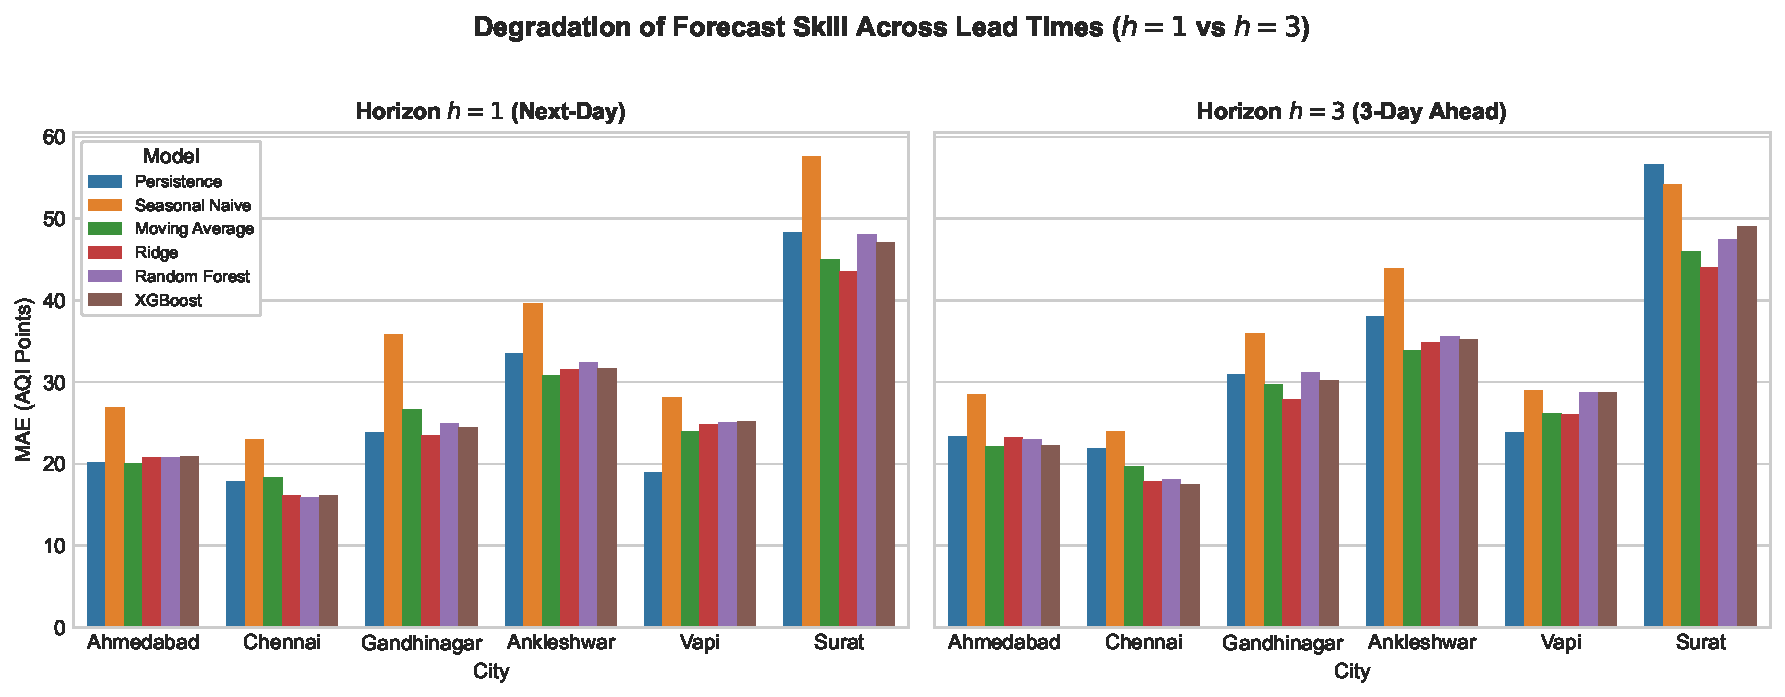
\includegraphics[width=0.88\textwidth]{../results/figures/fig5_horizon_decay.pdf}
  \caption{Horizon degradation from $h=1$ to $h=3$ across cities under Setup~C. Persistence error increases faster than multi-lag linear and moving-average models.}
  \label{fig:horizon_decay}
\end{figure}

As the forecast horizon extends to $h=3$, the predictive power of single-step persistence decays rapidly: in Gandhinagar, Persistence MAE degrades by $+29.6\%$ (from $23.88$ to $30.96$); in Vapi, it degrades by $+25.7\%$ (from $18.98$ to $23.86$). The 7-Day Moving Average and Seasonal Naive degrade by $-6\%$ to $+12\%$ (Surat Seasonal Naive even improves by $-6.0\%$). Ridge Regression degrades by $+1\%$ to $+19\%$, with Gandhinagar Ridge the worst case at $+19.0\%$. Tree ensembles span $-1\%$ to $+25\%$ (Surat Random Forest $-1.4\%$ to Gandhinagar Random Forest $+24.9\%$).

Consequently, machine learning models demonstrate nominally significant utility at extended lead times: in Gandhinagar at $h=3$, Ridge Regression achieved an MAE of \textbf{27.89} versus Persistence \textbf{30.96} ($+9.9\%$ skill, $p = 0.022$, Table~\ref{tab:dm_h3}); in Surat at $h=3$, Ridge achieved $\text{MAE} = \mathbf{44.05}$ versus Persistence \textbf{56.61} ($+22.2\%$ skill, $p = 0.024$, Table~\ref{tab:dm_h3}); and in Chennai the 7-Day Moving Average also reached significance ($p = 0.045$). However, only Chennai Ridge ($p = 0.0006$) and XGBoost ($p = 0.0002$) survive Bonferroni correction at $h=3$; Chennai Random Forest ($p = 0.0016$), Gandhinagar Ridge ($p = 0.022$), and Surat Ridge ($p = 0.024$) do not. Bonferroni-corrected skill is therefore confirmed only for Chennai at $h=3$. Moreover, at $h=3$ in Chennai, ARIMA(1,0,0) achieved $\text{MAE} = 21.13$ (no better than Persistence $21.87$, $p = 0.531$), whereas all three Chennai ML models significantly outperformed ARIMA(1,0,0) (Ridge $p = 0.0001$, Random Forest $p = 0.0009$, XGBoost $p < 0.0001$). Full $h=3$ Diebold-Mariano results for all cities and models are reported in Table~\ref{tab:dm_h3}.

\subsection{Diebold-Mariano Test Synthesis}
\label{sec:dm_synthesis}
The Diebold-Mariano $p$-values across all evaluated city and model configurations at $h=1$ under Setup~C are summarised in a heatmap (Figure~\ref{fig:diebold_mariano}), while full $h=3$ results appear in Table~\ref{tab:dm_h3}.

\begin{figure}[htbp]
  \centering
  \includegraphics[width=0.88\textwidth]{../results/figures/fig4_diebold_mariano.pdf}
  \caption{Diebold-Mariano test $p$-values comparing candidate forecasters to Persistence under Setup~C ($h=1$). Darker blue indicates smaller two-tailed $p$-values ($p < 0.05$ in either direction, i.e., either candidate superiority or Persistence dominance); lighter yellow indicates non-significant differences.}
  \label{fig:diebold_mariano}
\end{figure}

Across 60 pairwise comparisons (6 cities $\times$ 5 candidate models $\times$ 2 horizons), 12 configurations establish statistically significant differences ($p < 0.05$) in favour of the candidate model: 4 at $h=1$ (Ankleshwar Moving Average $p = 0.048$, and Chennai Ridge $p = 0.010$, Random Forest $p = 0.002$, and XGBoost $p = 0.001$) and 8 at $h=3$ (Ankleshwar Moving Average $p = 0.029$; Chennai Moving Average $p = 0.045$, Ridge $p = 0.0006$, Random Forest $p = 0.0016$, and XGBoost $p = 0.0002$; Gandhinagar Ridge $p = 0.022$; and Surat Moving Average $p = 0.020$ and Ridge $p = 0.024$; full $h=3$ breakdown in Table~\ref{tab:dm_h3}). Conversely, Persistence is statistically superior to candidate models in 12 configurations (10 at $h=1$ and 2 at $h=3$). In Vapi at $h=1$, Persistence outperforms all five candidate models: Seasonal Naive ($p = 7.3 \times 10^{-7}$), Moving Average ($p = 0.012$), Ridge ($p = 0.003$), XGBoost ($p = 0.0009$), and Random Forest ($p = 7.9 \times 10^{-5}$). Beyond Vapi, Persistence also beats Seasonal Naive in Ahmedabad ($p = 9.3 \times 10^{-9}$), Chennai ($p = 2.5 \times 10^{-6}$), Gandhinagar ($p = 5.1 \times 10^{-11}$), and Ankleshwar ($p = 0.015$), beats Moving Average in Gandhinagar ($p = 0.019$), and beats Seasonal Naive at $h=3$ in Ahmedabad ($p = 0.002$) and Gandhinagar ($p = 0.037$). Applying a conservative Bonferroni correction for the primary family of 60 candidate-vs-Persistence comparisons ($\alpha = 0.05 / 60 = 0.00083$), only 2 candidate wins survive (Chennai Ridge $p = 0.0006$ and XGBoost $p = 0.0002$ at $h=3$; Chennai ML models at $h=1$ under $k=0$ and Chennai Random Forest at $h=3$ do \emph{not} survive), while 5 Persistence wins survive under $k=0$ (Vapi Random Forest $p = 7.9 \times 10^{-5}$ and Seasonal Naive $p = 7.3 \times 10^{-7}$, plus Seasonal Naive in Ahmedabad, Chennai, and Gandhinagar; Vapi XGBoost at $p = 0.0009$ does \emph{not} survive, and the 5-win count depends on $k=0$ since Vapi Random Forest shifts to $p = 0.0058$ under $k=3$).

\textit{Note on DM bandwidth and sensitivity:} At $h=1$, the lag truncation is $k = h - 1 = 0$, meaning no autocorrelation correction is applied to the loss-differential variance; the DM test at $h=1$ reduces to a Harvey--Leybourne--Newbold small-sample corrected $t$-test on the loss differentials. At $h=3$, $k=2$ lags are used. To verify that our $h=1$ conclusions are not artefacts of $k=0$, we re-ran the DM test with lag truncation $k=3$ across all six cities. In Chennai, all three ML models remained statistically significant (Ridge $p = 0.008$, Random Forest $p = 0.0018$, and XGBoost $p = 0.00075$, which would survive the 0.00083 Bonferroni threshold under $k=3$); in Vapi, Persistence remained statistically superior to all ML models (Random Forest $p = 0.0058$, XGBoost $p = 0.0085$, Ridge $p = 0.038$), while Ankleshwar Moving Average ($p = 0.068$) and Gandhinagar Moving Average ($p = 0.069$) lost nominal significance.

\paragraph{Additional Baselines and Tuned-Model Sensitivity Check.}
Table~\ref{tab:extra_baselines} reports all four supplementary classical baselines (Climatology, Climatology+Persistence, ARIMA(1,0,0), and ETS) across all six cities under Setup~C ($h=1$).

\begin{table}[htbp]
\centering
\caption{Additional Classical Baselines at $h=1$ Under Setup~C (MAE, Skill vs.\ Persistence, and Two-Tailed DM $p$-Value). Asterisk ($^*$) denotes $p < 0.05$ in either direction (candidate win or Persistence win).}
\label{tab:extra_baselines}
\resizebox{0.9\linewidth}{!}{\begin{tabular}{llrrrc}
\toprule
City & Baseline & MAE & Pers.\ MAE & Skill & DM $p$-value \\
\midrule
Ahmedabad & Climatology & 34.70 & 20.21 & -0.717 & $<$0.0001$^*$ \\
 & Clim. + Pers. & 23.28 & 20.21 & -0.152 & 0.0002$^*$ \\
 & ARIMA(1,0,0) & 21.41 & 20.21 & -0.059 & 0.0177$^*$ \\
 & ETS (SES) & 27.63 & 20.21 & -0.367 & $<$0.0001$^*$ \\
Ankleshwar & Climatology & 39.24 & 33.53 & -0.171 & 0.0151$^*$ \\
 & Clim. + Pers. & 32.04 & 33.53 & +0.044 & 0.1047 \\
 & ARIMA(1,0,0) & 34.04 & 33.53 & -0.015 & 0.0115$^*$ \\
 & ETS (SES) & 35.60 & 33.53 & -0.062 & 0.6941 \\
Chennai & Climatology & 22.38 & 17.90 & -0.251 & $<$0.0001$^*$ \\
 & Clim. + Pers. & 17.25 & 17.90 & +0.036 & 0.1366 \\
 & ARIMA(1,0,0) & 16.96 & 17.90 & +0.052 & 0.0035$^*$ \\
 & ETS (SES) & 17.85 & 17.90 & +0.003 & 0.8198 \\
Gandhinagar & Climatology & 30.32 & 23.88 & -0.270 & $<$0.0001$^*$ \\
 & Clim. + Pers. & 22.44 & 23.88 & +0.060 & 0.1216 \\
 & ARIMA(1,0,0) & 22.64 & 23.88 & +0.052 & 0.0005$^*$ \\
 & ETS (SES) & 22.47 & 23.88 & +0.059 & 0.0460$^*$ \\
Surat & Climatology & 56.57 & 48.26 & -0.172 & 0.2542 \\
 & Clim. + Pers. & 45.56 & 48.26 & +0.056 & 0.1311 \\
 & ARIMA(1,0,0) & 42.13 & 48.26 & +0.127 & 0.0106$^*$ \\
 & ETS (SES) & 41.27 & 48.26 & +0.145 & 0.1501 \\
Vapi & Climatology & 39.94 & 18.98 & -1.104 & $<$0.0001$^*$ \\
 & Clim. + Pers. & 27.94 & 18.98 & -0.472 & $<$0.0001$^*$ \\
 & ARIMA(1,0,0) & 25.23 & 18.98 & -0.329 & 0.2915 \\
 & ETS (SES) & 31.42 & 18.98 & -0.656 & $<$0.0001$^*$ \\
\bottomrule
\end{tabular}}
\end{table}

Monthly Climatology performed substantially worse than Persistence in every city (all $p \le 0.0151$ except Surat $p = 0.254$), and Climatology+Persistence never significantly beat Persistence ($p \ge 0.105$ where its MAE was lower; it was significantly worse in Ahmedabad, $p = 0.0002$, and Vapi, $p < 0.0001$). ARIMA(1,0,0) and ETS failed to beat Persistence in Ahmedabad (ARIMA MAE $21.41, p = 0.018$; ETS $27.63, p < 0.0001$), Ankleshwar, and Vapi, while ETS gained significantly in Gandhinagar ($\text{MAE} = 22.47, p = 0.046$) and ARIMA(1,0,0) achieved statistically significant gains in Gandhinagar ($\text{MAE} = 22.64, p = 0.0005$, surviving even an 80-test Bonferroni threshold of $0.000625$), Surat ($\text{MAE} = 42.13, p = 0.011$), and Chennai ($\text{MAE} = 16.96, p = 0.0035$). In Gandhinagar and Surat, simple ARIMA(1,0,0) achieved lower MAE than every ML model in Table~\ref{tab:cross_city_mae}. Direct DM tests comparing ML against ARIMA(1,0,0) at $h=1$ show that in Gandhinagar ARIMA(1,0,0) significantly outperformed Random Forest ($p = 0.0022$) and XGBoost ($p = 0.0339$; vs.\ Ridge $p = 0.287$); in Surat differences were non-significant ($p \ge 0.228$); and in Chennai only Random Forest ($15.84$ vs.\ $16.96, p = 0.030$) significantly beat ARIMA(1,0,0) (Ridge $p = 0.112$, XGBoost $p = 0.064$). Finally, tuning hyperparameters on Ahmedabad via 3-fold \texttt{TimeSeriesSplit} on the initial training fold yielded Ridge ($\alpha=500$: MAE $21.03, p = 0.303$), Random Forest (\texttt{max\_depth=5, min\_samples\_leaf=5, n\_estimators=200}: MAE $20.22, p = 0.955$), and XGBoost (\texttt{lr=0.05, max\_depth=2, n\_estimators=200}: MAE $19.99, p = 0.734$). None significantly outperformed Persistence ($20.21$), confirming that ML underperformance in inland Gujarat is not an artefact of fixed default hyperparameters.

